% ===========================================================================
%  Final Review (16 Nov 2026): 23CSE498 Project Phase 2, Team 50
%
%  Compile from inside ppt/ (twice):
%      cd ppt && pdflatex -interaction=nonstopmode final_review.tex
%
%  NUMBERS: every measured figure is from paper revision 8, traced in
%  paper-draft/NUMBERS.md (section named in each slide's source tag), or from
%  the evidence file the tag names. Do not edit a number here without its
%  source. Figures 1 and 2 are the paper's own TikZ/pgfplots drawings.
%
%  House style (as ppt/sections_1_2_3.tex): no double or triple hyphens in
%  text (TikZ paths use `to`), no Oxford commas.
% ===========================================================================
\documentclass[aspectratio=169, 11pt]{beamer}

\usepackage[utf8]{inputenc}
\usepackage[T1]{fontenc}
\usepackage{xcolor}
\usepackage{booktabs}
\usepackage{array}
\usepackage{graphicx}
\usepackage{tikz}
\usetikzlibrary{calc,arrows.meta,positioning}
\usepackage{pgfplots}
\pgfplotsset{compat=1.16}

\graphicspath{{./}{../}{figures/}}
\IfFileExists{opensans.sty}{\usepackage[default,scale=0.95]{opensans}}{}

\definecolor{amritaMaroon}{HTML}{A4123F}
\definecolor{okGreen}{HTML}{2E7D32}
\definecolor{badRed}{HTML}{C62828}

\usetheme{Madrid}
\usecolortheme[named=amritaMaroon]{structure}
\setbeamertemplate{navigation symbols}{}
\setbeamertemplate{footline}[frame number]
\setbeamertemplate{headline}{}
\setbeamerfont{frametitle}{size=\normalsize}
\setbeamerfont{framesubtitle}{size=\tiny}
\setbeamercolor{block title}{bg=amritaMaroon!12,fg=amritaMaroon}
\setbeamercolor{block body}{bg=amritaMaroon!5}
\setbeamertemplate{itemize items}[circle]

% \src cites the artifact a number came from.
\newcommand{\src}[1]{{\color{gray}\tiny [#1]}}
\newcommand{\good}[1]{\textcolor{okGreen}{\textbf{#1}}}
\newcommand{\bad}[1]{\textcolor{badRed}{\textbf{#1}}}

\begin{document}

% ============================================================ TITLE
\begin{frame}
    \begin{tikzpicture}[remember picture,overlay]
        \node[fill=amritaMaroon, text=white, font=\bfseries\footnotesize, anchor=north east, rounded corners=2pt, inner sep=5pt]
        at ($(current page.north east) + (-0.2cm,-0.2cm)$)
        {Type 3: Software Project};
    \end{tikzpicture}

    \centering
    \IfFileExists{logo.png}{
\includegraphics[width=4.6cm]{logo.png}}{}
    \vspace{0.06cm}

    {\large \textbf{\textcolor{amritaMaroon}{What Catches a Lie That Works?}}}\\[1pt]
    {\footnotesize \textcolor{amritaMaroon}{Trust Scores, Anomaly Gates and Load-Misreporting Servers in Zero-Trust Edge Load Balancing}}\\[3pt]
    {\scriptsize Planned thesis title: \textit{Zero-Trust Load Balancing for Multi-Controller SDN in Edge Networks}}\\[3pt]
    {\footnotesize \textbf{23CSE498 Project Phase 2: Final Review} \quad | \quad \textbf{Team Number: 50}}\\
    \vspace{0.08cm}

    \begin{table}
        \centering
        \scriptsize
        \renewcommand{\arraystretch}{1.0}
        \begin{tabular}{|c|c|l|}
            \hline
            \textbf{S.No} & \textbf{Register Number} & \textbf{Student Name} \\
            \hline
            1 & CB.SC.U4CSE23262 & K R Jeevan Raj \\
            \hline
            2 & CB.SC.U4CSE23303 & Aravind Kumar M \\
            \hline
            3 & CB.SC.U4CSE23307 & Arjun Krishnakumar \\
            \hline
            4 & CB.SC.U4CSE23308 & Ashwin Kumar RM \\
            \hline
            5 & CB.SC.U4CSE23544 & Bhuvanesh S \\
            \hline
        \end{tabular}
    \end{table}
    \vspace{0.04cm}

    {\footnotesize Guide: \textbf{Dr. Radhika N}, Professor, Department of CSE} \\
    {\scriptsize 16 November 2026}
\end{frame}

% ============================================================ AGENDA
\begin{frame}{Agenda}
  \begin{columns}[T]
    \begin{column}{0.5\textwidth}
      \footnotesize
      \begin{enumerate}\itemsep5pt
        \item The problem: routing on what servers say
        \item What we built and how we measured it
        \item Architecture
        \item Results: the score, the gate and the threshold
        \item Results: the lie that works
        \item Results: witnesses beyond the score
      \end{enumerate}
    \end{column}
    \begin{column}{0.5\textwidth}
      \footnotesize
      \begin{enumerate}\itemsep5pt
        \setcounter{enumi}{6}
        \item Requirements met
        \item Defects we found in our own system
        \item Limitations
        \item Multi-controller: design and roadmap
        \item Live demonstration
      \end{enumerate}
    \end{column}
  \end{columns}
\end{frame}

% ============================================================ PROBLEM
\begin{frame}{The problem: routing on what servers say}
  \begin{columns}[T]
    \begin{column}{0.56\textwidth}
      \footnotesize
      \begin{itemize}\itemsep4pt
        \item Zero Trust (NIST SP 800-207) requires continuous verification but does not say how a control plane should verify the servers it sends work to.
        \item Edge load balancers rank servers on \textbf{self-reported} load. Trust-aware schemes add a trust score and a quarantine threshold.
        \item A server that misreports its load can attract traffic it then drops or serves slowly. Misreporting attacks on SDN load balancers are documented (Burke et al.\ 2023; Yu et al.\ 2024).
        \item \textbf{Our question:} which mechanism actually catches each kind of lie, and what does the lie gain before it is caught?
      \end{itemize}
    \end{column}
    \begin{column}{0.42\textwidth}
      \begin{block}{Attackers in every live run}
        \scriptsize
        \begin{tabular}{@{}ll@{}}
          srv3 & claims idle, is slow\\
          srv6 & blackhole (drops every task)\\
          srv1 & grayhole (drops half)\\
          srv8 & on-off (20 s period)\\
          iot37 & flooding client\\
          iot38 & spoofs iot1's identity\\
          iot39, iot40 & wrong key\\
        \end{tabular}
      \end{block}
      \scriptsize Staggered onsets from 15 s to 60 s, so each attack has a clean interval before it.
    \end{column}
  \end{columns}
\end{frame}

% ============================================================ WHAT WE BUILT
\begin{frame}{What we built}
  \begin{columns}[T]
    \begin{column}{0.5\textwidth}
      \footnotesize
      \textbf{Control plane} (Python, os-ken, OpenFlow 1.3)
      \begin{itemize}\itemsep2pt
        \item Trust score $T=\alpha\bar R+\beta\bar B+\gamma\bar H-\delta\bar A$ ranks servers; power-of-two choices with $\varepsilon$ exploration
        \item Anomaly gate: latency, timeout-rate and honesty tells
        \item Quarantine as OpenFlow drop rules; in-flight work re-steered; probation trials
        \item PRESENT-80 device admission with source-IP pinning
        \item Per-client meter throttle for floods
      \end{itemize}
    \end{column}
    \begin{column}{0.5\textwidth}
      \footnotesize
      \textbf{Witnesses beyond the score}
      \begin{itemize}\itemsep2pt
        \item \textbf{Switch witness:} switch byte counters joined with client reports; acts and holds
        \item \textbf{Attestation:} a sidecar measures the server agent before it is admitted
        \item \textbf{Replicated ledger:} 3 Raft replicas re-verify every trust record against the trust formula
        \item \textbf{Auditor:} a second, read-only controller (new for this review)
      \end{itemize}
      \textbf{Testbed:} Mininet, 8 edge servers, 40 IoT devices, 9 OVS switches; live dashboard
    \end{column}
  \end{columns}
\end{frame}

% ============================================================ METHOD
\begin{frame}{How we measured it}
  \footnotesize
  \begin{itemize}\itemsep4pt
    \item Every result is from \textbf{live runs} on the emulated network, about 300 s each, \textbf{five runs per arm}.
    \item From the liar experiment on, each batch was scored against a \textbf{prediction committed before it ran}; the outcome files record where a prediction failed.
    \item Continuous results: mean and two-sided 95\% Student-t interval over runs. Yes/no results: $k/n$ with a Wilson interval ($5/5 = [57\%, 100\%]$, $0/5 = [0\%, 43\%]$).
  \end{itemize}
  \vspace{4pt}
  \centering\scriptsize
  \begin{tabular}{@{}lrl@{}}
    \toprule
    Campaign & Runs & Question \\
    \midrule
    Ablation, threshold sweep, flood & 40 & which rail isolates whom, how fast \\
    Liar experiment & 80 & can a lie at honest speed win traffic \\
    Heterogeneous hardware & 30 & is an honest slow server mistaken for a liar \\
    Switch witness & 50 & can the switches name the lying party \\
    Attestation & 25 & does admission stop a tampered server \\
    Ledger re-verification & 20 & do replicas catch a forging controller \\
    Witness acting and holding & 83 & does acting on the switches restore service \\
    \midrule
    Total & 328 & plus one replicated-ledger run with a leader kill \\
    \bottomrule
  \end{tabular}\\[2pt]
  \src{paper-draft/NUMBERS.md}
\end{frame}

% ============================================================ ARCHITECTURE
\begin{frame}{Architecture}
  \centering
  \resizebox{\textwidth}{!}{%
  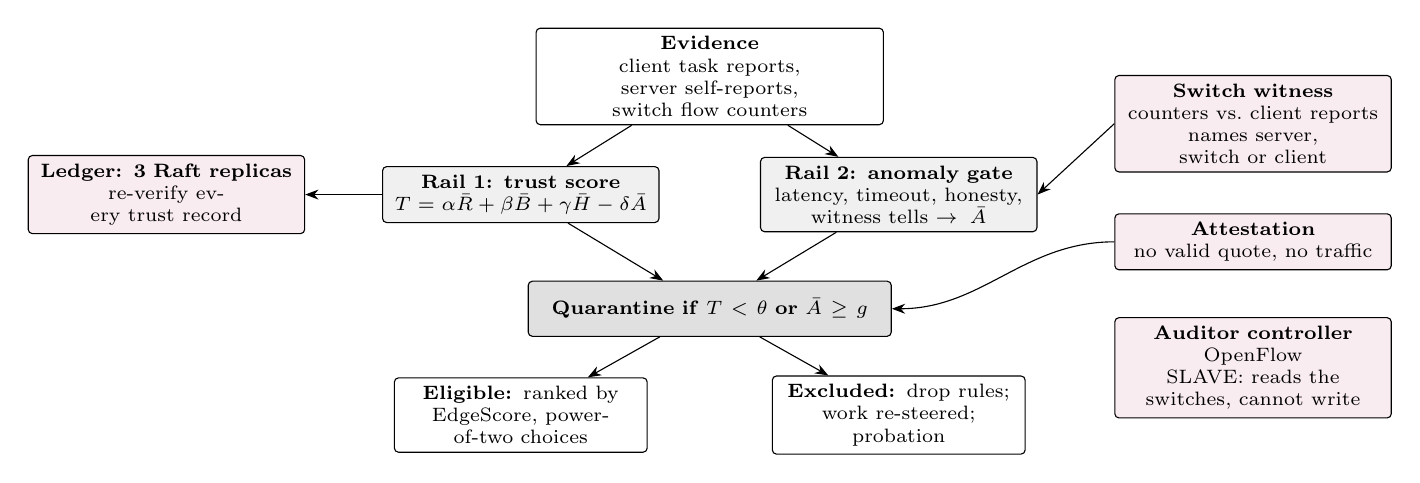
\begin{tikzpicture}[
    font=\scriptsize, >=Stealth,
    box/.style={draw, rounded corners=1.5pt, align=center, inner sep=3pt, minimum height=7mm},
    rail/.style={box, fill=black!6, text width=3.3cm},
    act/.style={box, text width=3.0cm},
    side/.style={box, fill=amritaMaroon!8, text width=3.3cm}]
    \node[box, text width=4.2cm] (ev) at (0,0) {\textbf{Evidence}\\ client task reports, server self-reports,\\ switch flow counters};
    \node[rail] (score) at (-2.4,-1.5) {\textbf{Rail 1: trust score}\\ $T=\alpha\bar R+\beta\bar B+\gamma\bar H-\delta\bar A$};
    \node[rail] (gate) at (2.4,-1.5) {\textbf{Rail 2: anomaly gate}\\ latency, timeout, honesty,\\ witness tells $\rightarrow \bar A$};
    \node[box, text width=4.4cm, fill=black!12] (dec) at (0,-2.95) {\textbf{Quarantine if} $T<\theta$ \textbf{or} $\bar A\ge g$};
    \node[act] (rank) at (-2.4,-4.3) {\textbf{Eligible:} ranked by EdgeScore, power-of-two choices};
    \node[act] (drop) at (2.4,-4.3) {\textbf{Excluded:} drop rules;\\ work re-steered; probation};
    \node[side] (wit) at (6.9,-0.6) {\textbf{Switch witness}\\ counters vs.\ client reports\\ names server, switch or client};
    \node[side] (att) at (6.9,-2.1) {\textbf{Attestation}\\ no valid quote, no traffic};
    \node[side] (led) at (-6.9,-1.5) {\textbf{Ledger: 3 Raft replicas}\\ re-verify every trust record};
    \node[side] (aud) at (6.9,-3.7) {\textbf{Auditor controller}\\ OpenFlow SLAVE: reads the\\ switches, cannot write};
    \draw[->] (ev) to (score); \draw[->] (ev) to (gate);
    \draw[->] (score) to (dec); \draw[->] (gate) to (dec);
    \draw[->] (dec) to (rank); \draw[->] (dec) to (drop);
    \draw[->] (wit.west) to (gate.east);
    \draw[->] (att.west) to[out=180, in=0] (dec.east);
    \draw[->] (score.west) to (led.east);
  \end{tikzpicture}}\\[6pt]
  \scriptsize The score \emph{ranks}; the gate \emph{excludes}, before ranking. The ablation arm removes only the gate's ability to act.
\end{frame}

% ============================================================ ABLATION
\begin{frame}{Result 1: the score never isolated the attackers that finish their tasks}
  \begin{columns}[T]
    \begin{column}{0.55\textwidth}
      \centering\scriptsize
      \begin{tabular}{@{}lccc@{}}
        \toprule
        Attacker & Crosses $\theta=0.30$ & \multicolumn{2}{c}{Quarantined} \\
                 & (all arms) & score only & both rails \\
        \midrule
        srv3 load misreport & \bad{0/15} & \bad{0/5} & \good{5/5} \\
        srv8 on-off         & \bad{0/15} & \bad{0/5} & \good{5/5} \\
        srv6 blackhole      & 15/15 & 5/5 & 5/5 \\
        srv1 grayhole       & 15/15 & 5/5 & 5/5 \\
        \bottomrule
      \end{tabular}\\[4pt]
      \src{NUMBERS.md, Tables II and III}
    \end{column}
    \begin{column}{0.43\textwidth}
      \footnotesize
      \begin{itemize}\itemsep4pt
        \item srv3 and srv8 complete their tasks, so their trust stays high: the gate quarantined them at $T = 0.710$ and $0.709$.
        \item Droppers lose work, so their score collapses: srv6 at $T = 0.130$, srv1 at $0.220$.
        \item Anomaly to quarantine: 3.5 to 12.5 ms over 20 node-runs.
      \end{itemize}
    \end{column}
  \end{columns}
  \vspace{6pt}
  \begin{block}{}
    \footnotesize Both rails are needed: the score handles servers that lose work; the gate handles servers that do the work badly.
  \end{block}
\end{frame}

% ============================================================ SWEEP
\begin{frame}{Result 2: a higher threshold lets the score isolate them, slowly}
  \begin{columns}[T]
    \begin{column}{0.56\textwidth}
      \centering
      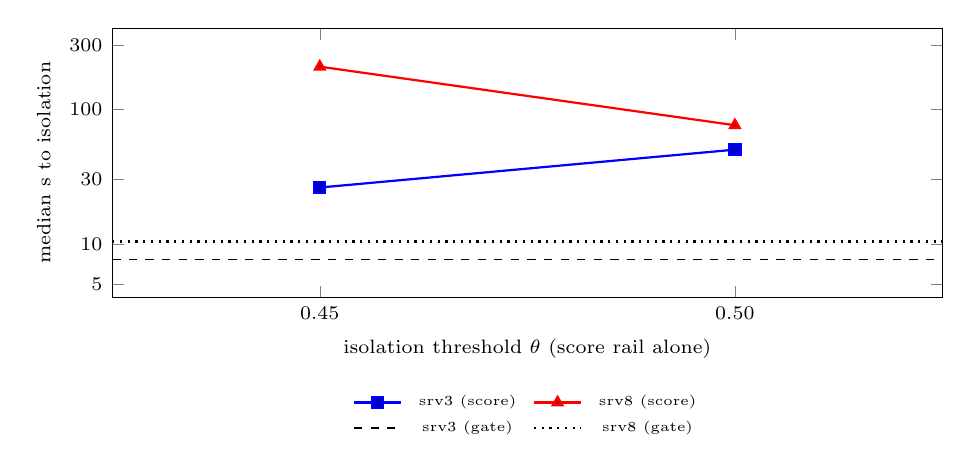
\begin{tikzpicture}
      \begin{axis}[
        width=\linewidth, height=5.0cm, ymode=log,
        xlabel={isolation threshold $\theta$ (score rail alone)},
        ylabel={median s to isolation}, xmin=0.425, xmax=0.525,
        xtick={0.45,0.50}, xticklabels={0.45,0.50}, ytick={5,10,30,100,300}, yticklabels={5,10,30,100,300},
        ymin=4, ymax=400, legend columns=2,
        legend style={font=\tiny, at={(0.5,-0.32)}, anchor=north, draw=none, column sep=4pt},
        tick label style={font=\scriptsize}, label style={font=\scriptsize}]
        \addplot+[mark=square*, thick] coordinates {(0.45,26.2) (0.50,50.1)};
        \addplot+[mark=triangle*, thick] coordinates {(0.45,207.3) (0.50,76.1)};
        \addplot[dashed, domain=0.425:0.525, samples=2] {7.6};
        \addplot[dotted, thick, domain=0.425:0.525, samples=2] {10.4};
        \legend{srv3 (score), srv8 (score), srv3 (gate), srv8 (gate)}
      \end{axis}
      \end{tikzpicture}
    \end{column}
    \begin{column}{0.42\textwidth}
      \footnotesize
      \begin{itemize}\itemsep4pt
        \item $\theta = 0.40$: srv3 0/5, srv8 1/5.
        \item $\theta = 0.45$: both 5/5, in a median 26.2 s and 207.3 s.
        \item $\theta = 0.50$: both 5/5, but one honest server and one attacker quarantined before its onset.
        \item The gate at $\theta = 0.30$: 7.6 s and 10.4 s, so the score is \textbf{3.4$\times$ to 20$\times$ slower}, inside a band a few hundredths wide.
      \end{itemize}
      \src{NUMBERS.md, \S VII-D}
    \end{column}
  \end{columns}
\end{frame}

% ============================================================ LIAR
\begin{frame}{Result 3: the lie that works}
  \footnotesize
  The ablation's attackers were slow, so the gate caught slowness. A liar at \textbf{honest speed}:\\[4pt]
  \centering\scriptsize
  \begin{tabular}{@{}llccc@{}}
    \toprule
    Liar & Routing on & Excess share (pts) & Quarantined & Median \\
    \midrule
    Consistent claims & raw claim & $-3.13$ & 5/5 & 8.2 s \\
    Adaptive (stealthy) & raw claim & $-1.16$ & 5/5 & 17.7 s \\
    \textbf{Split claim}: lies only in instantaneous load & raw claim & \bad{$+4.00$ [3.47, 4.52]} & \bad{0/5} & never \\
    Split claim & \textbf{verified} claim & \good{$+0.01$ [$-0.28$, $+0.30$]} & 3/5, 0.34\% of time & \\
    \bottomrule
  \end{tabular}\\[5pt]
  \raggedright\footnotesize
  \begin{itemize}\itemsep3pt
    \item The split claim keeps a truthful busy-time counter and lies in the one figure the router ranks on: it wins 4.0 points of traffic above its fair 12.5\% and is never caught.
    \item Ranking on the figure the controller \textbf{verifies} against busy time closes the gap at no measured honest cost: honest latency 396.2 ms vs.\ 396.4 ms. Verified routing is now the default.
    \item Fixing the liar checks cut honest false quarantines from 3.4 to 0.2 per run.
  \end{itemize}
  \src{NUMBERS.md, \S VII-E, Table 6; 80 runs, each batch against a prediction committed first}
\end{frame}

% ============================================================ HETEROGENEITY
\begin{frame}{Result 4: an honest slow server is not taken for a liar}
  \begin{columns}[T]
    \begin{column}{0.52\textwidth}
      \centering\scriptsize
      \begin{tabular}{@{}ll@{}}
        \toprule
        Arm (5 runs each) & Honest quarantines \\
        \midrule
        Mixed hardware, fleet median & \good{0} \\
        Mixed hardware, per-class baseline & \good{0} \\
        One server throttled to 25\% & \good{0} \\
        One server throttled to 10\% & 1 run of 5, 3.6 s \\
        \midrule
        Sybil on slow hardware & contained 5/5, 9.0 s \\
        Sybil on fast hardware & contained 5/5, 8.4 s \\
        \bottomrule
      \end{tabular}\\[4pt]
      \src{NUMBERS.md, \S VII-F}
    \end{column}
    \begin{column}{0.46\textwidth}
      \footnotesize
      \begin{itemize}\itemsep4pt
        \item The one false quarantine at 10\% came from a single slow status poll read as unreachable, then an inverted honesty check; the latency tell never fired.
        \item The attacker is still contained on either class of hardware.
      \end{itemize}
    \end{column}
  \end{columns}
\end{frame}

% ============================================================ WITNESS
\begin{frame}{Result 5: the switches name the lying party}
  \begin{columns}[T]
    \begin{column}{0.55\textwidth}
      \centering\scriptsize
      \begin{tabular}{@{}lcc@{}}
        \toprule
        Who lies (5 runs each) & First batch & After fixes \\
        \midrule
        Nobody & 0 blamed & \good{0 blamed} \\
        srv6 blackhole & 4/5 (53.9 s) & \good{5/5 (12.9 s)} \\
        srv1 grayhole & 5/5 (61.2 s) & \good{5/5 (14.1 s)} \\
        A switch hiding responses & 5/5 (14.1 s) & \good{5/5 (5.2 s)} \\
        Two badmouthing clients & 5/5 & \good{5/5 (12.0 s)} \\
        srv6 with a covering switch & srv6 5/5 & srv6 5/5; switch 0/5 \\
        \midrule
        Honest parties blamed & \bad{3 of 25 runs} & \good{0 of 25 runs} \\
        \bottomrule
      \end{tabular}\\[4pt]
      \src{NUMBERS.md, \S VII-G, Table 7}
    \end{column}
    \begin{column}{0.43\textwidth}
      \footnotesize
      \begin{itemize}\itemsep4pt
        \item Offline first: switch and client accounts agree to 0.9992 per honest server-run over 110 archived recordings.
        \item An honest task is 6 packets, 548 bytes in and 598 bytes back; "requests in, no full response out" is the drop tell.
        \item Two fixes: judge each party on its recent connections, and blame a client only when its switch-mates look clean.
        \item A switch covering for a dropper is the stated limit: the dropper is still named.
      \end{itemize}
    \end{column}
  \end{columns}
\end{frame}

% ============================================================ ATTESTATION
\begin{frame}{Result 6: attestation stops a tampered server before it serves}
  \begin{columns}[T]
    \begin{column}{0.60\textwidth}
      \centering\scriptsize
      \begin{tabular}{@{}lccc@{}}
        \toprule
         & Tampered, & Tampered, & Runtime attack, \\
         & no attestation & attestation & attestation \\
        \midrule
        Admitted & n/a & \good{0/5} & 5/5 \\
        Connections served & 17 [8, 25] & \good{0} & 20 [15, 24] \\
        Contained (median) & 10.9 s & never needed & 9.9 s \\
        Honest timeouts & 24.6 & \good{0.0} & 27.6 \\
        Honest success (\%) & 99.52 & 99.98 & 99.48 \\
        \bottomrule
      \end{tabular}\\[4pt]
      \src{NUMBERS.md, \S VII-H, Table 8}
    \end{column}
    \begin{column}{0.38\textwidth}
      \footnotesize
      \begin{itemize}\itemsep4pt
        \item Attestation measures code at load time; an attack that starts at runtime passes it 5/5 and is caught by behaviour instead.
        \item Cost: the fleet is admitted within 4.1 s; a quote is verified in a median 0.20 ms.
        \item The two mechanisms cover different attacks; neither replaces the other.
      \end{itemize}
    \end{column}
  \end{columns}
\end{frame}

% ============================================================ LEDGER
\begin{frame}{Result 7: ledger replicas catch a forged score, not forged evidence}
  \begin{columns}[T]
    \begin{column}{0.55\textwidth}
      \centering\scriptsize
      \begin{tabular}{@{}lcc@{}}
        \toprule
        The controller forges srv3's & score & evidence \\
        \midrule
        Forged records rejected & \good{5,478 / 5,482} & \bad{0 / 3,787} \\
        Honest records rejected & 0 & 0 \\
        srv3 route share after onset & 23.9\% & 23.6\% \\
        \quad (before onset) & 13.2\% & 12.5\% \\
        Honest task success & 99.98\% & \bad{82.58\%} \\
        Commit per block (median) & 9.5 ms & 9.7 ms \\
        \bottomrule
      \end{tabular}\\[4pt]
      \src{NUMBERS.md, \S VII-I, Table 9; evidence/ledger}
    \end{column}
    \begin{column}{0.43\textwidth}
      \footnotesize
      \begin{itemize}\itemsep4pt
        \item Replicas replay the trust arithmetic on every record. A forged \textbf{score} fails the replay and is rejected within a median 0.22 s.
        \item The ledger \textbf{detects}; it does not stop the controller routing on the forged score.
        \item Forged \textbf{evidence} produces arithmetic that checks out. It passes the replicas and blinds the controller's own detectors.
        \item Only the switch witness saw it: 5/5 runs, median 11.1 s.
      \end{itemize}
    \end{column}
  \end{columns}
\end{frame}

% ============================================================ WITNESS ACTS
\begin{frame}{Result 8: acting on the switches restores service}
  \begin{columns}[T]
    \begin{column}{0.58\textwidth}
      \centering\scriptsize
      \begin{tabular}{@{}lccc@{}}
        \toprule
        Forging controller; & Time quarantined & Connections & Honest \\
        the witness... & (\%) & after onset & success (\%) \\
        \midrule
        observes & 0 & 770 & \bad{82.24} \\
        acts & 84.0 & 135 & 97.68 \\
        acts and holds & 95.3 & 64 & \good{99.06} \\
        \midrule
        no attacker, holds & & & 99.99 \\
        \bottomrule
      \end{tabular}\\[4pt]
      \src{NUMBERS.md, \S VII-J, Table 10}
    \end{column}
    \begin{column}{0.40\textwidth}
      \footnotesize
      \begin{itemize}\itemsep4pt
        \item \textbf{Acts:} a blamed server raises the gate's witness signal; quarantined in a median 11.0 s.
        \item \textbf{Holds:} it stays out until the witness sees it serve 3 trial connections in a row.
        \item Closes 87\% (acts) and 95\% (holds) of the gap to the no-attacker run.
        \item After the trial-path fixes: 245 of 245 trials judged, none charged to another server.
      \end{itemize}
    \end{column}
  \end{columns}
\end{frame}

% ============================================================ FLOOD + NFR
\begin{frame}{Requirements met}
  \begin{columns}[T]
    \begin{column}{0.54\textwidth}
      \centering\scriptsize
      \begin{tabular}{@{}lll@{}}
        \toprule
        Requirement & Target & Measured \\
        \midrule
        Routing decision & $<200$ ms & mean 0.54 to 0.55 ms \\
                         &           & p95 0.71 to 0.73 ms \\
        Isolation & $<3$ s & re-dispatch 12.9 to 23.5 ms \\
        Ledger overhead & $<15\%$ & 0.045 to 0.052\% \\
        Raft commit$^{*}$ & $<500$ ms & mean 14.06 ms, p95 20.24 ms \\
        \bottomrule
      \end{tabular}\\[4pt]
      {\tiny First three rows: the five both-rails runs. $^{*}$The replicated-ledger run below.}\\ \src{NUMBERS.md, \S VII-N}\\[6pt]
      \begin{block}{Leader killed mid-run}
        \scriptsize New leader in 0.47 s; 649 blocks submitted, 649 committed, none dropped; the restarted replica caught up in 1.0 s.
      \end{block}
    \end{column}
    \begin{column}{0.44\textwidth}
      \footnotesize
      \textbf{Flood throttle} (meter in the switch)\\[2pt]
      \centering\scriptsize
      \begin{tabular}{@{}lcc@{}}
        \toprule
         & off & on \\
        \midrule
        Honest latency, mean & 105.0 ms & \good{91.7 ms} \\
        Honest latency, p95 & 177.7 ms & \good{139.4 ms} \\
        Tasks served to flooder & 8,951 & \good{292.8} \\
        Honest devices throttled & & \good{0} \\
        \bottomrule
      \end{tabular}\\[4pt]
      \src{NUMBERS.md, \S VII-L, Table 12}
    \end{column}
  \end{columns}
\end{frame}

% ============================================================ DEFECTS
\begin{frame}{Defects we found in our own system, and fixed}
  \scriptsize\renewcommand{\arraystretch}{1.2}
  \begin{tabular}{@{}>{\raggedright\arraybackslash}p{0.25\textwidth}>{\raggedright\arraybackslash}p{0.40\textwidth}>{\raggedright\arraybackslash}p{0.29\textwidth}@{}}
    \toprule
    Defect & Evidence & After the fix \\
    \midrule
    Quarantine was an absorbing state & isolated servers kept trust near 0.18 while provably healthy, with no traffic to recover on & probation trials; the gate is never relaxed \\
    Servers charged for tasks they never received & re-steered tasks counted against the new server & 123 of 32,107 reports (0.38\%) now uncharged \\
    Liar checks fired on honest servers & 3.4 honest false quarantines per run & 0.2 per run \\
    Witness slow and occasionally wrong & droppers named after 53.9 and 61.2 s; honest parties blamed in 3 of 25 runs & 12.9 to 14.1 s; 0 of 25 \\
    Probation trials black-holed, then their tails mis-charged & 43 misattributed reports, 34 to honest servers & 245/245 trials judged, 0 misattributed \\
    \bottomrule
  \end{tabular}\\[6pt]
  \footnotesize
  The trial-path defects explain the three honest trust dips (0.417 to 0.421) in the threshold sweep: each came within a second of a misattributed timeout. One earlier claim, that faster containment means worse attack labelling, was \textbf{withdrawn}: Spearman $\rho = -0.522$, $p = 0.122$, $n = 10$.\\
  \src{NUMBERS.md, \S VIII-A, \S VIII-B, \S IX}
\end{frame}

% ============================================================ LIMITATIONS
\begin{frame}{Limitations}
  \footnotesize
  \begin{itemize}\itemsep5pt
    \item \textbf{Emulated data plane.} Mininet on one 4-core laptop; timings depend on that host. One flood run was excluded because the host suspended mid-run.
    \item \textbf{Five runs per arm.} A 5/5 result has a Wilson interval of [57\%, 100\%].
    \item \textbf{Scripted adversaries.} One adaptive liar; no adversary that learns the detectors' thresholds.
    \item \textbf{The ledger detects, it does not prevent.} The controller still routes on a forged score, and forged evidence passes the replicas.
    \item \textbf{The witness's one false action}, in the last 25-run batch: an honest server quarantined for 26 s after a machine-wide stall. Persistence for witness strikes is designed but not built.
    \item \textbf{One controller.} Every result above has a single controller; the second is read-only so far.
    \item \textbf{Scale.} 8 servers and 40 devices live; larger fleets only in simulation.
  \end{itemize}
\end{frame}

% ============================================================ MULTI-CONTROLLER
\begin{frame}{Multi-controller: what runs today and what comes next}
  \begin{columns}[T]
    \begin{column}{0.48\textwidth}
      \begin{block}{Running for this review}
        \scriptsize
        \begin{itemize}\itemsep2pt
          \item \textbf{Auditor controller}: joins every switch as OpenFlow SLAVE, which the switch enforces as read-only. It cannot install or delete a rule.
          \item It reads the server off the rewrite the switch applies, not the primary's label, and judges it from counters alone: request bytes in, no full response out.
          \item The ledger replicas run on separate laptops.
        \end{itemize}
      \end{block}
      \scriptsize Demo scene: the primary forges srv3's evidence with its witness off. Its own panel shows srv3 healthy; the auditor shows srv3 not serving.
    \end{column}
    \begin{column}{0.50\textwidth}
      \footnotesize
      \textbf{Next, each with a prediction registered first}
      \begin{enumerate}\itemsep2pt
        \item \textbf{Fencing:} the primary claims MASTER with a generation ID held in the Raft cluster.
        \item \textbf{Takeover:} the auditor is promoted, restores trust state from the replicas' replay and seeds quarantines from the flow tables.
        \item \textbf{Arms:} no false takeover; primary crash (outage, lost tasks, quarantines kept); forging primary (detection and takeover time, honest success recovered).
        \item Then the open plan items: witness strike persistence with a stall-injection arm; scale and percentile switch lies; the eBPF kernel witness.
      \end{enumerate}
      \scriptsize Literature check on multi-controller and BFT SDN comes first, to state exactly what is new.
    \end{column}
  \end{columns}
\end{frame}

% ============================================================ DEMO
\begin{frame}{Live demonstration}
  \begin{columns}[T]
    \begin{column}{0.47\textwidth}
      \centering\scriptsize
      \begin{tabular}{@{}ll@{}}
        \toprule
        Laptop & Role \\
        \midrule
        A & primary controller, Mininet data plane \\
        B, C, D & ledger replicas n1, n2, n3 \\
        E & auditor controller, viewer \\
        \bottomrule
      \end{tabular}\\[4pt]
      \raggedright\scriptsize
      The data plane is emulated on laptop A; the control plane is spread across laptops over a phone hotspot.
    \end{column}
    \begin{column}{0.51\textwidth}
      \footnotesize
      \begin{enumerate}\itemsep2pt
        \item Normal routing across all 8 servers
        \item Wrong key and spoof refused at admission
        \item Load-misreporting server caught by the gate
        \item Droppers caught and held by the witness
        \item Flooding client throttled in the switches
        \item A replica laptop closed: the ledger keeps committing
        \item A forging primary, exposed by the auditor
      \end{enumerate}
      \scriptsize If the network fails on the day, the same scenes are replayed from rehearsal recordings.
    \end{column}
  \end{columns}
\end{frame}

% ============================================================ REFERENCES
\begin{frame}{Key references}
  \scriptsize
  \begin{enumerate}\itemsep2pt
    \item S.\ Rose, O.\ Borchert, S.\ Mitchell and S.\ Connelly, \textit{Zero Trust Architecture}, NIST SP 800-207, 2020.
    \item M.\ Huang, Z.\ Li, F.\ Xiao, S.\ Long and A.\ Liu, ``Trust mechanism-based multi-tier computing system for service-oriented edge-cloud networks,'' \textit{IEEE TDSC}, 21(4), pp.\ 1639-1651, 2024.
    \item B.\ Ali, M.\ A.\ Gregory and S.\ Li, ``Trust-aware task load balancing in multi-access edge computing based on blockchain and a zero trust security capability framework,'' \textit{Trans.\ Emerging Telecommunications Technologies}, 34(12), e4845, 2023.
    \item Q.\ Burke, P.\ McDaniel, T.\ La Porta, M.\ Yu and T.\ He, ``Misreporting attacks against load balancers in software-defined networking,'' \textit{Mobile Networks and Applications}, 28(4), pp.\ 1482-1497, 2023.
    \item M.\ Yu, Q.\ K.\ Burke, T.\ La Porta and P.\ McDaniel, ``Stealthy misreporting attacks against load balancing,'' \textit{IEEE/ACM Trans.\ Networking}, 32(4), pp.\ 3622-3635, 2024.
    \item M.\ Dhawan, R.\ Poddar, K.\ Mahajan and V.\ Mann, ``SPHINX: Detecting security attacks in software-defined networks,'' \textit{NDSS}, 2015.
    \item M.\ Mitzenmacher, ``The power of two choices in randomized load balancing,'' \textit{IEEE TPDS}, 12(10), pp.\ 1094-1104, 2001.
    \item D.\ Ongaro and J.\ Ousterhout, ``In search of an understandable consensus algorithm,'' \textit{USENIX ATC}, pp.\ 305-319, 2014.
    \item P.\ Huang et al., ``Gray failure: The Achilles' heel of cloud-scale systems,'' \textit{HotOS}, 2017.
    \item B.\ Lantz, B.\ Heller and N.\ McKeown, ``A network in a laptop: Rapid prototyping for software-defined networks,'' \textit{ACM HotNets}, 2010.
  \end{enumerate}
\end{frame}

\begin{frame}
  \centering
  \vspace{1.5cm}
  {\Large \textcolor{amritaMaroon}{\textbf{Thank you}}}\\[10pt]
  \footnotesize Questions
\end{frame}

\end{document}
